\chapter{Разработка программного комплекса}

В данной главе будет описан процесс разработки программного комплекса, который позволяется смоделировать и  построить оптимальный порядок перегрузки реактора.

\section{Описание архитектуры программного комплекса}

Программный комплекс для моделирования и построения оптимального порядка перезагрузки реактора представляет собой модульное веб-приложение, состоящие из веб-интерфейса управления и 3 модулей: сервис хранения состояний, сервис расчета порядка и сервис моделирования.
Каждый модуль предоставляет интерфейс прикладного программирования (API), который работает по схеме передачи репрезентативного состояния. 
То есть каждый модуль является отдельным REST-сервисом.
Данные между сервисами передаются в формате JSON.

Такая архитектура позволяет развернуть программный комплекс в облачных сервисах PaaS и IaaS.
При этом будет достигнута возможность горизонтального масштабирования программного комплекса при необходимости.

\subsection{Сервис хранения состояний}

Сервис хранения состояний представляет собой хранилище ТА-моделей.
Пользователь имеет возможность создания, чтения, редактирования и удаления ТА-моделей.
Таким образом сервис хранения состояния является персистентным хранилищем моделей, предоставляемых пользователем.

ТА-модель в сервисе задается как кортеж из пяти элементов: множество состояний, множество операций, множество допустимых переходов, начальное состояние и множество конечных состояний.
Каждое состояние имеет свое название и словарь дополнительных данных.
Каждая операция также имеет свое название и словарь дополнительных данных.

Cервис хранения состояний имеет следующие методы REST API (см. таблицу~\ref{tab:automata}).
\begin{table} [htbp]
  \centering
  \parbox{15cm}{\caption{Методы API сервиса хранения состояния}\label{tab:automata}}
  \begin{center}
  \begin{tabular}{| l | l | p{0.5\linewidth} |}
  \hline
  Адрес & HTTP-метод & Выполняемое действие\\
  \hline
  api/automata & GET & Получить список всех автоматов\\
  \hline
  api/automata & POST & Добавить новое описание автомата (из JSON-данных запроса)\\
  \hline
  api/automata/<id> & GET & Получить описание автомата номер <id>\\
  \hline
  api/automata/<id> & PUT & Изменить описание автомата номер <id> (из JSON-данных запроса)\\
  \hline
  api/automata/<id> & DELETE & Получить описание автомата номер <id>\\
  \hline
  \end{tabular}
  \end{center}
\end{table}
Пример работы API приведен в приложении~\ref{json:automata}.

Архитектура сервиса представлена на рис.~\ref{pic:automata-arch}.
Поступающие HTTP-запросы обрабатываются HTTP-сервером фреймворка Flask.
В зависимости от типа запроса расширение Flask-RESTful API маршрутизирует запросы на соответствующий парсер запроса.
Каждый парсер изменяет модель данных в соответствии с запросом.
При изменении модели данных ORM фреймворк SQLAlchemy производит синхронизацию данных модели и данных в базе данных.
При этом SQLAlchemy может работать с большинством современных СУБД без изменения программного кода.

\begin{figure}[ht]
\center{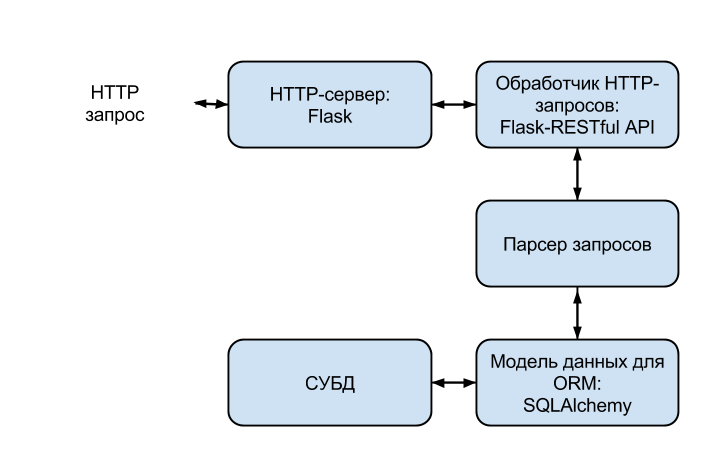
\includegraphics[width=0.65\linewidth]{automata-arch}}
\caption{Архитектура сервиса хранения состояний}
\label{pic:automata-arch}
\end{figure}

\subsection{Сервис расчета порядка}

Сервис расчета порядка представляет собой расчетный сервис для поиска оптимального порядка действий для достижения одного из конечных состояний ТА-модели.
В качестве входных данных используется объект ТА-модели, переданный сервисом хранения состояний.
Выходными данными является список действий для перехода из начального состояния автомата в одно из конечных состояний.

В качестве расчетной основы используется библиотека NetworkX, реализующая высокоэффективную модель графа и алгоритм поиска A*.

Cервис расчета порядка имеет следующие методы REST API (см. таблицу~\ref{tab:pathfinder}).
\begin{table} [htbp]
  \centering
  \parbox{15cm}{\caption{Методы API сервиса расчета порядка}\label{tab:pathfinder}}
  \begin{center}
  \begin{tabular}{| l | l | p{0.5\linewidth} |}
  \hline
  Адрес & HTTP-метод & Выполняемое действие\\
  \hline
  api/pathfinder & POST & Найти оптимальные пути в автомате (описание автомата в JSON-данных запроса)\\
  \hline
  \end{tabular}
  \end{center}
\end{table}

Пример работы API приведен в приложении~\ref{json:pathfinder}.

Архитектура сервиса представлена на рис.~\ref{pic:pathfinder-arch}.
Поступающие HTTP-запросы обрабатываются HTTP-сервером фреймворка Flask.
Расширение Flask-RESTful API маршрутизирует запросы на парсер автомата.
Парсер автомата преобразует JSON-представление автомата в объект графа библиотеки NetworkX.
Затем вызывается алгоритм поиска А* для объекта графа.
Полученный результат возвращается в HTTP-ответе.

\begin{figure}[ht]
\center{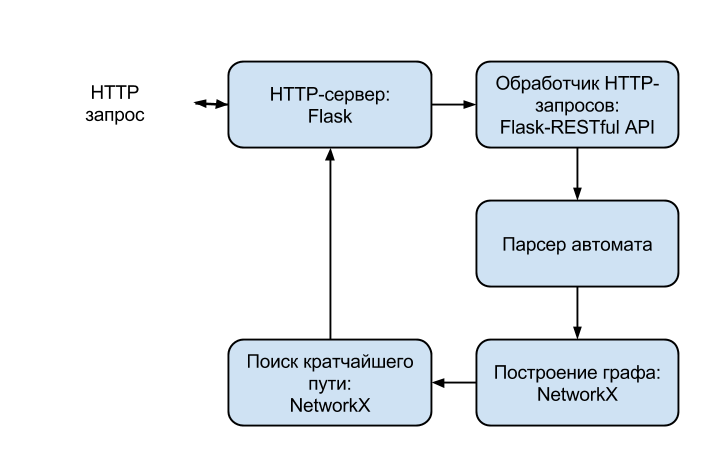
\includegraphics[width=0.65\linewidth]{pathfinder-arch}}
\caption{Архитектура сервиса расчета порядка}
\label{pic:pathfinder-arch}
\end{figure}

\subsection{Сервис моделирования состояний}
Сервис моделирования состояний представляет собой набор искусственных нейронных сетей и их обучающие выборки.
Пользователь может создать нейронную сеть, указав параметры (количество слоев, количество нейронов в каждом слое и функции активации нейронов) и задав обучающую выборку.
После обучения на вход ИНС можно подать входной вектор (в том числе ТА-модель) и получить отклик, который соответствует аппроксимированному значению обучающей выборки.

В качестве расчетной основы используется библиотека PyBrain, реализующая различные модели искусственных нейронных сетей, а также хранилище обучающих выборок и алгоритмы обучения.

Cервис моделирования состояний имеет следующие методы REST API (см. таблицу~\ref{tab:neuronnetwork}).
\begin{table} [htbp]
  \centering
  \parbox{15cm}{\caption{Методы API моделирования состояний}\label{tab:neuronnetwork}}
  \begin{center}
  \begin{tabular}{| l | l | p{0.6\linewidth} |}
  \hline
  Адрес & HTTP-метод & Выполняемое действие\\
  \hline
  api/neuronnetwork & POST & Задать нейронную сеть и обучающую выборку (описание в JSON-данных запроса)\\
  \hline
  api/neuronnetwork & GET & Получить отклик нейронной сети (входной вектор в данных запроса)\\
  \hline
  \end{tabular}
  \end{center}
\end{table}

Архитектура сервиса представлена на рис.~\ref{pic:neuronnetwork-arch}.
Поступающие HTTP-запросы обрабатываются HTTP-сервером фреймворка Flask.
Расширение Flask-RESTful API маршрутизирует запросы на парсер нейронной сети или на уже обученную нейронную сеть.
Парсер нейронной преобразует JSON-представление в объект нейронной сети библиотеки PyBrain и его обучающую выборку. 
При этом производится обучение нейронной сети до конвергенции.
Для обученной сети может быть получен отклик на входной вектор.
Полученный результат возвращается в HTTP-ответе.

\begin{figure}[ht]
\center{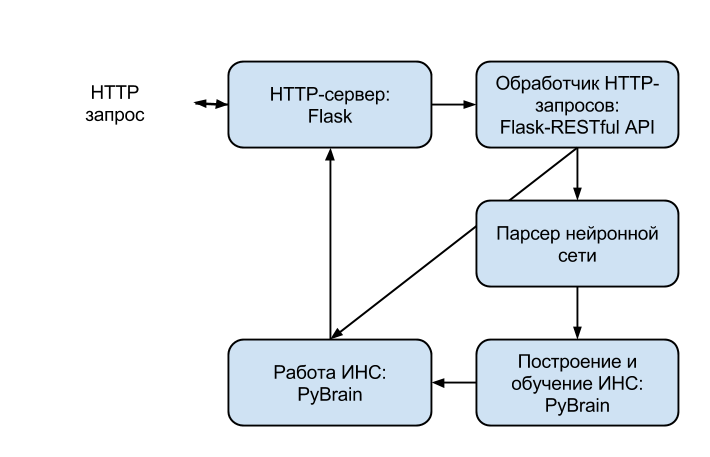
\includegraphics[width=0.65\linewidth]{neuronnetwork-arch}}
\caption{Архитектура сервиса моделирования состояния}
\label{pic:neuronnetwork-arch}
\end{figure}

\section{Технологии, используемые при разработке программного комплекса}
\subsection{Python}
Python --- высокоуровневый язык программирования общего назначения, ориентированный на повышение производительности разработчика и читаемости кода. 
Синтаксис ядра Python минималистичен. 
В то же время стандартная библиотека включает большой объём полезных функций.

Python поддерживает несколько парадигм программирования, в том числе структурное, объектно-ориентированное, функциональное, императивное и аспектно-ориентированное. 
Основные архитектурные черты --- динамическая типизация, автоматическое управление памятью, полная интроспекция, механизм обработки исключений, поддержка многопоточных вычислений и удобные высокоуровневые структуры данных. 
Код в Питоне организовывается в функции и классы, которые могут объединяться в модули (они в свою очередь могут быть объединены в пакеты).

Python портирован и работает почти на всех известных платформах --- от КПК до мейнфреймов. 
Существуют порты под Microsoft Windows, практически все варианты UNIX (включая FreeBSD и Linux), Plan 9, Mac OS и Mac OS X, iPhone OS 2.0 и выше, Palm OS, OS/2, Amiga, HaikuOS, AS/400 и даже OS/390, Windows Mobile, Symbian и Android.

Python --- стабильный и распространённый язык. 
Он используется во многих проектах и в различных качествах: как основной язык программирования или для создания расширений и интеграции приложений. 
На Python реализовано большое количество проектов, также он активно используется для создания прототипов будущих программ. 
Python используется во многих крупных компаниях.
Python с пакетами NumPy, SciPy и MatPlotLib активно используется как универсальная среда для научных расчётов в качестве замены распространенным специализированным коммерческим пакетам Matlab, IDL и др.\cite{python-main}

\subsection{Flask}
Flask является микрофреймворком для создания веб-приложений на языке Python
<<Микро>> не означает, что ваше веб-приложение целиком помещается в один файл с кодом на Python, хотя конечно же это может быть и так. 
Также, это не означает, что Flask испытывает недостаток функциональности. 
<<Микро>> в слове <<микрофреймворк>> означает, что Flask стремится придерживаться простого, но расширяемого ядра. 
Flask не может решить многие вещи, например, какую базу данных использовать. 
А те решения, которые он может принять, например, который из движков для работы с шаблонами использовать, легко изменить. 

По умолчанию, Flask не включает уровень абстракции баз данных, валидации форм или каких-то иных, для чего уже существуют различные занимающиеся этим библиотеки. 
Вместо этого, Flask поддерживает расширения для добавления подобной функциональности в ваше приложение, таким образом, как если бы это было реализовано в самом Flask. 
Многочисленные расширения обеспечивают интеграцию с базами данных, валидацию форм, обработку загрузок на сервер, различные открытые технологии аутентификации и так далее. 
Flask может быть <<микро>>, но при этом он готов для использования в реальных задачах для самых разнообразных нужд.

\subsection{REST}

REST (сокр. англ. Representational State Transfer, <<передача состояния представления>> или <<передача репрезентативного состояния>>) --- стиль построения архитектуры распределенного приложения. 
Был описан и популяризован в 2000 году Роем Филдингом (Roy Fielding), одним из создателей протокола HTTP. 
Самой известной системой, построенной в значительной степени по архитектуре REST, является современная Всемирная паутина.

Данные в REST должны передаваться в виде небольшого количества стандартных форматов (например HTML, XML, JSON). 
Сетевой протокол (как и HTTP) должен поддерживать кэширование, не должен зависеть от сетевого слоя, не должен сохранять информацию о состоянии между парами <<запрос-ответ>>. 
Утверждается, что такой подход обеспечивает масштабируемость системы и позволяет ей эволюционировать с новыми требованиями.

\subsection{SQLAlchemy}

SQLAlchemy --- это программная библиотека на языке Python для работы с реляционными СУБД с применением технологии ORM.
Служит для синхронизации объектов Python и записей реляционной базы данных. 
SQLAlchemy позволяет описывать структуры баз данных и способы взаимодействия с ними на языке Python без использования SQL. 
Библиотека была выпущена в феврале 2006 под лицензией открытого ПО MIT.

Использование SQLAlchemy для автоматической генерации SQL-кода имеет несколько преимуществ по сравнению с ручным написанием SQL:
\begin{itemize}
 \item [-] Безопасность. 
 Параметры запросов экранируются, что делает атаки типа внедрение SQL-кода маловероятными.
 \item [-] Производительность. 
 Повышается вероятность повторного использования запроса к серверу базы данных, что может позволить ему в некоторых случаях применить повторно план выполнения запроса.
 \item [-] Переносимость. 
 SQLAlchemy, при должном подходе, позволяет писать код на Python, совместимый с несколькими back-end СУБД.
 Несмотря на стандартизацию языка SQL, между базами данных имеются различия в его реализации, абстрагироваться от которых и помогает SQLAlchemy. \cite{sqlalchemy}
\end{itemize}

\subsection{NetworkX}
Библиотека networkX создана на языке Python и предназначена для работы с графами и другими сетевыми структурами. 
Это свободное ПО распространяемое под новой BSD лицензией.

Основные возможности библиотеки:
\begin{itemize}
 \item [-] Классы для работы с простыми, ориентированными и взвешенными графами;
 \item [-] Узлом может быть практически что угодно: time-series, текст, изображение, XML;
 \item [-] Сохранение / загрузка графов в/из наиболее распространённых форматов файлов хранения графов;
 \item [-] Встроенные процедуры для создания графов базовых типов;
 \item [-] Методы для обнаружения подграфов, клик и К-дольных графов (K-core) ( максимальный подграф в котором каждая вершина имеет по крайней мере уровень К ).
 \item [-] Получение таких характеристик графа как степени вершин, высота графа, диаметр, радиус, длинны путей, центр, промежуточности, и т. д.;
 \item [-] Визуализировать сети в виде 2D и 3D графиков.
\end{itemize}

Заявляется, что библиотека свободно может оперировать весьма большими сетевыми структурами, уровня графа с 10 миллионами узлов и 100 миллионами дуг между ними. 
В виду того, что он базируется на низкоуровневой структуре данных языка Python под названием «словарь-словарей», память расходуется эффективно, графы хорошо масштабируются, мало зависят от особенностей операционной системы в которой выполняется скрипт и отлично подходят для популярного на данный момент направления по анализу данных из социальных сетей и графов.\cite{networkx-habr}

\subsection{PyBrain}

PyBrian представляет собой модульную библиотеку предназначенную для реализации различных алгоритмов машинного обучения на языке Python. Основной его целью является предоставление исследователю гибких, простых в использовании, но в то же время мощных инструментов для реализации задач из области машинного обучения, тестирования и сравнения эффективности различных алгоритмов.
Название PyBrain является аббревиатурой от английского: Python-Based Reinforcement Learning, Artificial Intelligence and Neural Network Library.
Как сказано на одном сайте: PyBrain --- это швейцарский армейский нож в области нейро-сетевых вычислений. 

Библиотека построена по модульному принципу, что позволяет использовать её как студентам для обучения основам, так и исследователям, нуждающимся в реализации более сложных алгоритмов. 
Общая структура процедуры её использования приведена на следующей схеме (см. рис.~\ref{pic:pybrain}).\cite{schaul2010}
\begin{figure}[ht]
\center{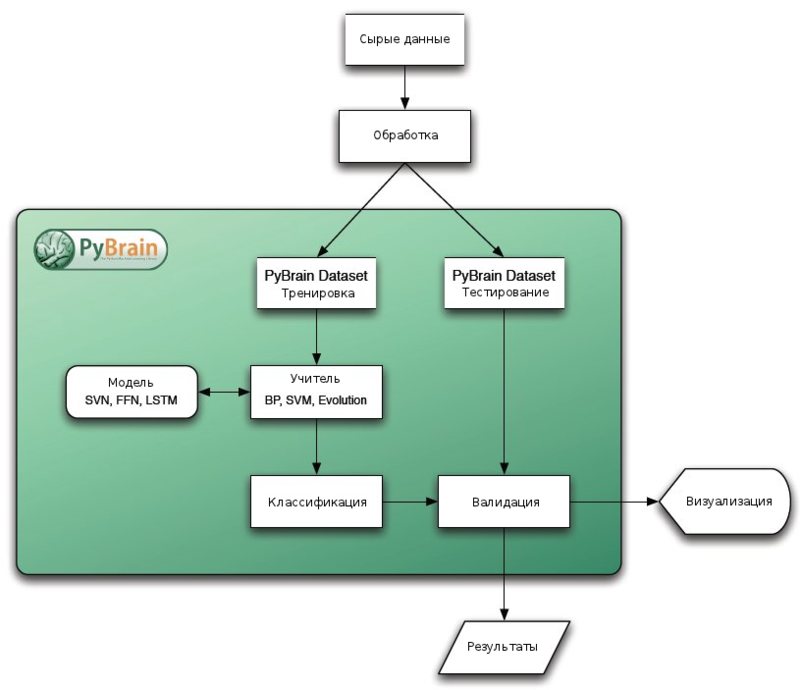
\includegraphics[width=0.65\linewidth]{pybrain}}
\caption[Процедура использования библиотеки PyBrain]{Процедура использования библиотеки PyBrain}
\label{pic:pybrain}
\end{figure}

\subsection{Облачные вычисления}

Облачные вычисления (англ. cloud computing)--- это модель обеспечения повсеместного и удобного сетевого доступа по требованию к общему пулу (англ. pool) конфигурируемых вычислительных ресурсов (например, сетям передачи данных, серверам, устройствам хранения данных, приложениям и сервисам — как вместе, так и по отдельности), которые могут быть оперативно предоставлены и освобождены с минимальными эксплуатационными затратами и/или обращениями к провайдеру. 

Потребители облачных вычислений могут значительно уменьшить расходы на инфраструктуру информационных технологий (в краткосрочном и среднесрочном планах) и гибко реагировать на изменения вычислительных потребностей, используя свойства вычислительной эластичности (англ. elastic computing) облачных услуг.

Платформа как услуга  (PaaS, англ. PaaS or Platform as a Service) --- модель предоставления облачных вычислений, при которой потребитель получает доступ к использованию информационно-технологических платформ: операционных систем, систем управления базами данных, связующему программному обеспечению, средствам разработки и тестирования, размещённым у облачного провайдера. 
В этой модели вся информационно-технологическая инфраструктура, включая вычислительные сети, серверы, системы хранения, целиком управляется провайдером, провайдером же определяется набор доступных для потребителей видов платформ и набор управляемых параметров платформ, а потребителю предоставляется возможность использовать платформы, создавать их виртуальные экземпляры, устанавливать, разрабатывать, тестировать, эксплуатировать на них прикладное программное обеспечение, при этом динамически изменяя количество потребляемых вычислительных ресурсов.

Провайдер облачной платформы может взимать плату с потребителей в зависимости от уровня потребления, тарификация возможна по времени работы приложений потребителя, по объёму обрабатываемых данных и количеству транзакций над ними, по сетевому трафику. 
Провайдеры облачных платформ достигают экономического эффекта за счёт использования виртуализации и экономии на масштабах, когда из множества потребителей в одно и то же время лишь часть из них активно использует вычислительные ресурсы, потребители — за счёт отказа от капитальных вложений в инфраструктуру и платформы, рассчитанных под пиковую мощность и непрофильных затрат на непосредственное обслуживание всего комплекса.

Инфраструктура как услуга (IaaS, англ. IaaS or Infrastructure-as-a-Service) предоставляется как возможность использования облачной инфраструктуры для самостоятельного управления ресурсами обработки, хранения, сетями и другими фундаментальными вычислительными ресурсами, например, потребитель может устанавливать и запускать произвольное программное обеспечение, которое может включать в себя операционные системы, платформенное и прикладное программное обеспечение. 
Потребитель может контролировать операционные системы, виртуальные системы хранения данных и установленные приложения, а также ограниченный контроль набора доступных сервисов (например, межсетевой экран, DNS). 
Контроль и управление основной физической и виртуальной инфраструктурой облака, в том числе сети, серверов, типов используемых операционных систем, систем хранения осуществляется облачным провайдером.\cite{cloud-comp}

%\section{Пример работы программного комплекса}